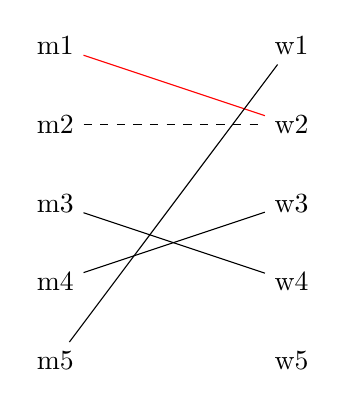
\begin{tikzpicture}[black/.style={circle,draw,fill=black,inner sep=0pt, minimum width=4pt}]
\node at (1,4) (m1) {m1};
\node at (1,3) (m2) {m2};
\node at (1,2) (m3) {m3};
\node at (1,1) (m4) {m4};
\node at (1,0) (m5) {m5};
\node at (4,4) (w1) {w1};
\node at (4,3) (w2) {w2};
\node at (4,2) (w3) {w3};
\node at (4,1) (w4) {w4};
\node at (4,0) (w5) {w5};

\draw (m3) -- (w4);
\draw (m4) -- (w3);
\draw[red] (m1) -- (w2);
\draw (m5) -- (w1);
\draw[dashed] (m2) -- (w2);
\end{tikzpicture}
